% % % % % % % % % % % % % % 
% 
% Skript zu NUMERIK I
% WS14/15
% von Prof. Dr. Blank
% Universität Regensburg
% 
% 
%	Kap. 9: Lineare Gleichungssysteme: Iterative Methoden
% 
% % % % % % % % % % % % % % 


\chapter{Lineare Gleichungssysteme: Iterative Methoden}
\sectione{Einführung}
\begin{Bspe}[Approximation der Poisson-Gleichung]\label{9.1.1}
  Betrachte $\Delta u=u_{xx}-u_{yy}\eqqcolon f$ in $\Omega=(0,1)^2$
mit $u=0$ auf $\delta\Omega$
\begin{figure}
  \begin{image}{Gitter mit Unbekannten zu Beispiel \ref{9.1.1}}
    \begin{tikzpicture}[scale=0.8]
     \foreach \xy/\num in
     {0/0,1/1,2/2,3/3,13/N-2,14/N-1,15/N,16/N+1}
       {
         %outer x lines
         \draw (\xy,16) -- (\xy,0) node[anchor=north] {$x_{\num}$};
         % outer y lines
         \draw (16,\xy) -- (0,\xy) node[anchor=east] {$y_{\num}$};
       }
       \foreach \xy/\num in
       {6,7,8,9,10}
       {
         % inner x lines
         \draw (\xy,4.5) -- (\xy,11.5);
         \draw (4.5,\xy) -- (11.5,\xy);
       }

       %points
       \foreach \xy/\val in {1/-1,0/\phantom{-}2}
       {
         \fill[color=blue] (8,8+\xy) circle[radius=2pt]
         node[anchor=south west] {\small\val};
         \fill[color=red] (8+\xy,8) circle[radius=2pt]
         node[anchor=north west] {\small\val};
       }
       \fill[color=blue] (8,8-1) circle[radius=2pt]
       node[anchor=north west] {\small -1};
       \fill[color=red] (8-1,8) circle[radius=2pt]
       node[anchor=north west] {\small -1};
       \fill[color=blue] (8,8) ++(0:2pt) arc (0:180:2pt);

       \draw[->] (8,-0.5) -- (8,-2.5);
       \draw[color=blue] (8,-3) node {-1};
       \draw[color=blue] (8,-5) node {-1};
       \draw[color=red] (7,-4) node {-1};
       \draw[color=red] (9,-4) node {-1};
       \draw (8,-4) node {4};
 \end{tikzpicture}
\end{image}
\end{figure}
Es gibt $N^2$ Unbekannte, $N^2\times N^2$.
Also $A\in\R^{n\times n}$ mit $n=N^2$.
\begin{gather*}
  (x_0,y_0),(x_1,y_0),(x_2,y_0),
  \ldots,(x_{N+1},y_0),(x_0,y_1),(x_1,y_1),
  \ldots,(x_{N+1},y_{N+1})\\
  \Rightarrow 0\ldots0~\underbrace{-1~0\ldots0~-1}_{N}~4~
  \underbrace{-1~0\ldots0~-1}_{N}~0\ldots0
  \qquad \text{$i$-te Zeile von $A$}
\end{gather*}
Damit sind nur maximal 5 Elemente verschieden von Null je Zeile
und $Au$ benötigt ca. $5n=5N^2$ Multiplikationen (statt $n^2=N^4$).
\begin{gather}
  A=
  \begin{pmatrix}
    A_{11}&-I&&0\\
    -I &\ddots &\ddots \\
    && &-I\\
    0&&-I&A_{nn}    
  \end{pmatrix}
  \quad \text{mit }
  A_{ii}=\begin{pmatrix}
    4&-1\\
    -1&\ddots&\ddots\\
    &&&-1\\
    &&-1&4
  \end{pmatrix}\in\R^{n\times n}
\label{IX.1.2}
\end{gather}
\end{Bspe}

\subsectione{Typische Aufgabenstellung}
Zu lösen ist $Ax=b$ mit
\begin{itemize}
\item $A\in\R^{n\times n}$, $n$ sehr groß
\item $A$ dünn besetzt
\item $A$ hat Blockstruktur
\end{itemize}
s. Folien

\sectione{Klassische (stationäre) Verfahren}
Betrachte
\begin{gather}
  Ax=b
\label{IX.2.1}
\end{gather}
Wähle nun für $A$ eine \textbf{Aufspaltung} $A=M-N$
mit einer einfach invertierbaren Matrix $M$, s.d.
\begin{gather}
  Mx = Nx +b \label{IX.2.2}
\end{gather}

Die \textbf{Iterationsvorschrift} ist dann: 
Löse zu einem gegebenen Startwert $x^{(0)}$ als Schätzung für $x$
für $k=0,-1,2, \ldots$
\begin{gather}
  Mx^{(k+1)}= Nx^{(k)} +b \label{IX.2.3}
\end{gather}
Es ergeben sich folgende Äquivalenzen
\begin{align}
  \eqref{IX.2.3} &\Leftrightarrow
                   x^{(k+1)} = M^{-1}Nx^{(k)}+M^{-1}b 
                   \label{IX.2.4}\\
                 &\Leftrightarrow x^{(k+1)} = x^{(k)} + M^{-1}r^{(k)}
                   \label{IX.2.5}
\end{align}
mit $r^{(k)}= b-Ax^{(k)}$ (Residuum im $k$-ten Schritt).

Als \textbf{Abbruchkriterium}
\begin{enumerate}[a)]
\item sollte immer eine maximale Iterationszahl angegeben werden und
\item wird oft für eine gegebene Toleranz $tol\geq\nn{r^{(k)}}$
  oder wie diskutiert $tol\cdot \nn{b}\geq \nn{r^{(k)}}$ verwendet.
\end{enumerate}

Nach \eqref{IX.2.4} ergibt sich also die \textbf{Fixpunktiteration}
\begin{gather}
  x^{(k+1)} = Gx^{(k)} +d \eqqcolon g(x^{(k)})
  \label{IX.2.6}
\end{gather}
zur \textbf{Fixpunktgleichung}\index{Fixpunktgleichung}
\begin{gather*}
  x^{*} = Gx^{*} + d = g(x^{*})
\end{gather*}
mit der \textbf{Iterationsmatrix} 
\begin{gather}
  G=M^{-1}N=I-M^{-1}A = g'(x)
  \label{IX.2.7}
\end{gather}
und $d=M^{-1}b$. Weiterhin folgt
\begin{gather*}
  x^{(k+1)}-x^{*} = G(x^{(k)}-x^{*})=G^{k+1}(x^{(0)}-x^{*})
\end{gather*}
und hiermit gilt elementweise (falls $x^{(0)}-x^{*}\not\in ker
(G^{k+1})$)
\begin{gather*}
  \lim_{k\to\infty} x^{(k)} = x^{*}
  \quad\Leftrightarrow\quad
  \lim_{k\to\infty} G^k =0
\end{gather*}


\begin{Satze}[Konvergenzkriterien]\label{9.2.1}
  Sei $G\in\R^{n\times n}$.
Dann sind folgende Aussagen äquivalent:
\begin{enumerate}[i)]
\item Die Iteration \eqref{IX.2.6} konvergiert für jeden Startwert
  $x^{(0)}\in\R^n$
\item Es gilt $\lim_{k\to\infty}G^k = 0$
\item Für den Spektralradius 
  $\rho(G) \coloneqq \max_i|\lambda_i|$ 
  mit $\lambda_i\in\C$ Eigenwert zu $G$ gilt
  \begin{gather}
    \rho(G) < 1
    \label{IX.2.8}
  \end{gather}
\end{enumerate}

\begin{proof}
  \begin{description}
  \item[i)$\Leftrightarrow$ ii):] siehe oben.
  \item[ii)$\Rightarrow$ iii):]  Ist $\rho(G)\geq 1$ dann 
existiert ein Eigenwert $\lambda\in\C$ mit $|\lambda|>1$ und
Eigenvektor $v\neq 0$ zu $G$.
Damit ist $G^kv=\lambda^kv$. 
Mit $\lim_{k\to\infty}\lambda^k\neq 0$ (falls existent) folgt
$\lim_{k\to\infty}G^k \neq 0$.
\item[iii)$\Rightarrow$ ii):] Sei $\rho(G)<1$.
  Da $\left(TGT^{-1}\right)^k = TG^kT^{-1}$
 für eine invertierbare Matrix $T$, reicht es,
für die Jordansche Normalform $J=TGT^{-1}$ von $G$ zu zeigen,
dass $\lim_{k\to\infty}J^k=0$ gilt.
Da $ J^k =
\begin{pmatrix}
  J_1^k && 0 \\
  &\ddots \\
  0&& J_m^k
\end{pmatrix}$ mit den Jordankästchen
$J_i =
\begin{pmatrix}
  \lambda_i & 1 && 0\\
  &\ddots&\ddots\\
  &&&1\\
  0&&&\lambda_i
\end{pmatrix} \eqqcolon \lambda_iI+S_i$
mit $S_i =
\begin{pmatrix}
  0&1&&0 \\
  &\ddots&\ddots\\
  &&&1\\
  0&&&0
\end{pmatrix}$ ist, ist nur $\lim_{k\to\infty}J_i^k$ zu untersuchen.
\begin{align*}
  J_i^k &= (\lambda_i I+S_i)^k \\
        &= \sum_{l=0}^{k}\begin{pmatrix}k\\l\end{pmatrix}
  \lambda_i^{k-l} S_i^l\\
        &=\sum_{l=0}^{n-1} \begin{pmatrix}k\\l\end{pmatrix}
  \lambda_i^{k-l} S_i^{k}
\end{align*}
für $k\geq n$, da für $S_i\in\R^{r\times r}$ gilt $S_i^r=0$ 
und mit $r\leq k$ ist dann $\lim_{k\to\infty}S_i^k=0$.
Weiterhin gilt $\begin{pmatrix}k\\l\end{pmatrix}\leq k^l$ 
und wegen $|\lambda_i|<1$
\begin{gather*}
  \left| \begin{pmatrix}k\\l\end{pmatrix}\right|
  \cdot\left|\lambda_i^{k-l}\right|
  \leq \left|\lambda_i^{k}\right| 
  \cdot \left|\frac{k}{\lambda_i}\right|^l
  \leq \left|\lambda_i\right|^k
  \cdot \left|\frac{k}{\lambda_i}\right|^n
\overset{\mathclap{k\rightarrow \infty}}{\longrightarrow} 0
\end{gather*}
Also $J_i^k\longrightarrow 0$ für $k\longrightarrow \infty$.
  \end{description}
\end{proof}
\end{Satze}


\begin{Leme}
  Für jede von einer Vektornorm induzierten Matrixnorm 
$\nn{\bullet}$ gilt
\begin{gather}
  \rho(G) \leq \nn{G}
\label{IX.2.9}
\end{gather}
\begin{proof}
  Sei $\lambda$ Eigenwert von $G$ zum Eigenvektor $v$.
Dann gilt $\frac{\nn{Gv}}{\nn{v}} = |\lambda|$
und daraus folgt direkt
\begin{gather*}
  \nn{G} \geq \sup_{v\in V}\frac{\nn{Gv}}{\nn{v}}\geq |\lambda|
  \quad \forall \lambda
\end{gather*}
\end{proof}
\end{Leme}

$\nn{G}<1$ ist meist leichter zu prüfen als $\rho(G)<1$.
Desweiteren gilt die Fehlerabschätzung
\begin{gather}
   \nn{x^{(k)}-x^{*}}\leq \nn{G}^k\nn{x^{(0)}-x^{*}}
   \label{IX.2.10}
\end{gather}
für submultiplikative Matrixnormen.


%-----------------------------------

\marginpar{24.01.2015}
\sectione{Gesamt- und Einzelschritt-Verfahren}
In \eqref{IX.2.3} soll $M$ leicht \enquote{invertierbar} sein.

\subsectione{Richardson-Verfahren}\index{Richardson-Verfahren}
Es sei $M=I$, also $G=I-A$ und
$x^{(k+1)}=x^{(k)}+(b-Ax^{(k)})=x^{(k)}+r^{(k)}$
konvergiert für alle Startwerte genau dann, wenn
\begin{gather}
  \rho(G) = \max_i\left| 1-\lambda_i \right|<1
\label{IX.3.1}
\end{gather}
mit den Eigenwerten $\lambda_i$ zu $A$.
Es muss also gelten $\rho(A) <2$, was selten der Fall ist.

\begin{image}{Mögliche Werte der $\lambda_i$ für $M=I$}
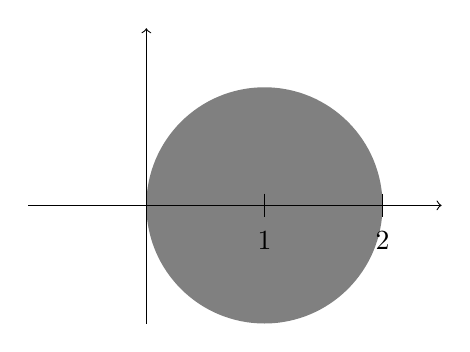
\begin{tikzpicture}[scale=1.5]
  \fill[color=gray] (1,0) circle[radius=1cm]; 
  \draw[->] (0,-1) -- (0,1.5);
  \draw[->] (-1,0) -- (2.5,0);
  \draw (1,0.1) -- (1,-0.1) ++(0,-0.2) node(anchor above) {1};
  \draw (2,0.1) -- (2,-0.1) ++(0,-0.2) node(anchor above) {2};
  \draw (2.25,1.25) node {$\C$};
\end{tikzpicture}
\end{image}

\subsectione{Gesamtschritt- oder Jacobi-Verfahren}
\index{Jacobi-Verfahren}
Es sei $M_G\coloneqq D$ die Diagonale von $A$.

\textbf{Vorsicht:} Falls $a_{ii}=0$ für ein $i$, 
permutiere die Zeilen oder Spalten.
Für ein reguläres $A$ gibt es eine Permutation,
so dass  $D$ anschließend invertierbar ist.

Es gilt die Rekursionsvorschrift
\begin{gather}
  x^{(k+1)}=x^{(k)}+D^{-1}r^{(k)}
\label{IX.3.2}
\end{gather}
Oft wird die Schreibweise mit $A=L+D+R$ =
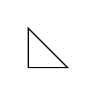
\begin{tikzpicture}
  \draw (0,0) -- (0,0.5) -- (0.5,0) --(0,0);
\end{tikzpicture}
+
\begin{tikzpicture}
  \draw (0.5,0) -- (0,0.5);
\end{tikzpicture}
+
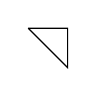
\begin{tikzpicture}
  \draw (0,0.5) -- (0.5,0.5) --(0.5,0) -- (0,0.5);
\end{tikzpicture}~
benutzt
\begin{gather}
  Dx^{(k+1)}= -(L+R)x^{(k)}+b
\label{IX.3.3}
\end{gather}
bzw. für $i=1,\ldots,n$
\begin{gather}
  a_{ii}x_i^{(k+1)} = -\sum_{j\neq i}a_{ij}x_j^{(k)}+b_i
\label{IX.3.4}
\end{gather}
Die Iterationsmatrix ist $G_G\coloneqq -D^{-1}(L+R)$.


\subsectione{Einzelschritt- oder Gauß-Seidel-Verfahren}
\index{Gauß-Seidel-Verfahren}
Falls in \eqref{IX.3.4} die Schleife von $i=1$ bis $i=n$
sukzessive durchlaufen wird, stehen bei der Berechnung von
$x_i^{(k+1)}$ die Werte $x_1^{(k+1)},\ldots,x_{i-1}^{(k+1)}$
bereits zur Verfügung und können genutzt werden.
Also gilt für $i=1,\ldots,n$
\begin{align}
  &&a_{ii}x_i^{(k+1)} & = -\sum_{j=1}^{i-1}a_{ij}x_j^{(k)}
                        -\sum_{j=1+1}^{n}a_{ij}x_j^{(k)}+ b_i
                        \label{IX.3.5} \\\nonumber
  &\Longleftrightarrow &Dx^{(k+1)}&=-Lx^{(k+1)}-Rx^{(k)}+b \\
  &\Longleftrightarrow &(D+L)x^{(k+1)}&=-Rx^{(k)}+b
                                    \label{IX.3.6} \\\nonumber
  &\Longleftrightarrow &x^{(k+1)} &= x^{(k)}+(D+L)^{-1}r^{(k)}
\end{align}
Daraus folgt, dass $M_G=D+L$, $N=-R$ 
und die zugehörige Iterationsmatrix ist 
\begin{gather*}
  G_E = -(D+L)^{-1}R = -(D+L)^{-1}A+I
\end{gather*}

\begin{Bspe}
  Ohne zusätzliche Voraussetzungen an $A$ lässt sich
  nicht voraussagen, welches der beiden Verfahren konvergiert.
  \begin{align*}
    A&= \begin{pmatrix}
      1&-2&2\\
      -1&1&-1\\
      -2&-2&1
    \end{pmatrix}
    &\Longrightarrow \rho(G_G)&=0, &\rho(G_E)&=2(1+\sqrt{2})\\
    A&= \frac{1}{2}\begin{pmatrix}
      2&1&1\\
      -2&2&-2\\
      -1&1&2
    \end{pmatrix}
    &\Longrightarrow \rho(G_G)&=\frac{1}{2}\sqrt{5}, &\rho(G_E)&=\frac{1}{2}
  \end{align*}
\end{Bspe}

\begin{Defe}~
  \begin{enumerate}[a)]
  \item $A\in\R^{n\times n}$ erfüllt die \textbf{starke Zeilensummenbedingung}
    \index{Zeilensummenbedingung!stark}, 
    bzw. $A\in\R^{n\times n}$ ist strikt diagonaldominant, wenn
    \begin{gather}
      |a_{ii}|>\sum_{j\neq i} |a_{ij}| \quad 1\leq i\leq m
      \label{IX.3.7}
    \end{gather}
  \item $A$ erfüllt die \textbf{schwache Zeilensummenbedingung}
    \index{Zeilensummenbedingung!stark}, 
    bzw. $A\in\R^{n\times n}$ ist schwach diagonaldominant, wenn
    \begin{gather}
      |a_{ii}|\geq \sum_{j\neq i} |a_{ij}| \quad 1\leq i\leq m
      \label{IX.3.8}
    \end{gather} 
    und für zumindest ein $i$ die starke Bedingung erfüllt ist.
  \end{enumerate}
\end{Defe}

\begin{Defe}
  $A\in\R^{n\times n}$ heißt \textbf{zerfallend}\index{Matrix!zerfallend},
  wenn es $J\subsetneqq \{1,\ldots,n\}$ gibt,
  so dass $a_{ij}=0$ für $i\in J, j\not\in J$.
\end{Defe}

\begin{Beme}
  Falls $A$ zerfallend ist, gibt es eine Permutationsmatrix $P$, 
  so dass
  \begin{gather*}
    P^TAP = \begin{pmatrix}
      \widetilde{A}_{11}&0\\
      \widetilde{A}_{21}&\widetilde{A}_{22}
    \end{pmatrix}
  \end{gather*}
mit $\widetilde{A}_{11}\in\R^{p\times p}$,
$\widetilde{A}_{22}\in\R^{q\times q}$,
$p,q>0$, $p+q=m$.
Das Gleichungssystem $Ax=b$ zerfällt somit in zwei kleinere
\begin{align*}
  \widetilde{A}_{11}\widetilde{x}_1 &= \widetilde{b}_1\\
  \widetilde{A}_{22}\widetilde{x}_2 &= \widetilde{b}_2
                                      -\widetilde{A}_{21}\widetilde{x}_1
\end{align*}
\end{Beme}

\begin{Bspe}
  Die Matrix $A$ in Beispiel \ref{9.1.1} zur Approximation der
  Poisson-Gleichung ist schwach und nicht stark diagonal dominant und
  ist nicht zerfallend.
\end{Bspe}

\begin{Satze}[Zeilensummenkriterium]\index{Zeilensummenkriterium}
  \label{9.3.9}
  Das Jacobi- sowie Gauß-Seidel-Verfahren konvergiert, falls 
  \begin{enumerate}[a)]
  \item $A$ die starke Zeilensummenbedingung erfüllt.
  \item $A$ die schwache Zeilensummenbedingung erfüllt und nicht
    zerfallend ist.
  \end{enumerate}
In beiden Fällen gilt
\begin{gather}
  \nn{G_E}_\infty \leq \nn{G_G}_\infty 
  = \max_i\frac{1}{|a_{ii}|}\sum_{j\neq i} |a_{ij}|
  \eqqcolon \overline{a} \leq 1
  \label{IX.3.9}
\end{gather}
\begin{proof}
  Es ist $G_G\coloneqq D^{-1}(L+R) = D^{-1}(A-D)$ und damit 
  $\overline{a}=\nn{G}_\infty\leq 1$ aufgrund der Diagonaldominanz.
  Für das Einzelschrittverfahren betrachte 
    $y\coloneqq G_E x=-(D+L)^{-1}Rx$, wofür gilt
$Dy = -Ly-Rx$. Dann
\begin{align*}
  |(G_Ex)_1| = |y_1| &\leq \frac{1}{|a_{11}|}\left(
                       \sum_{j=2}^{n}|a_{1j}|\cdot |x_j|
                       \right) \\
                     &\leq \nn{x}_\infty \frac{1}{|a_{11}|}\left(
                       \sum_{j=2}^{n}|a_{1j}|
                       \right) \\
                     &\leq \nn{x}_\infty \overline{a}\\
                     &\leq \nn{x}_\infty
\end{align*}
Rekursiv folgt aus $|y_j|\leq \nn{x}_\infty $ für $j\leq i-1$
\begin{align}\nonumber
  |(G_Ex)_i| = |y_i| &\leq \frac{1}{|a_{ii}|}\left(
                       \sum_{j=1}^{i-1}|a_{ij}|
                       \cdot \underbrace{|y_j|}_{\mathclap{\leq\nn{x}_\infty}}
                       +\sum_{j=i+1}^{n}|a_{ij}|
                       \cdot \underbrace{|x_j|}_{\mathclap{\leq\nn{x}_\infty}}
                       \right)\\\nonumber
                     &\leq \nn{x}_\infty \frac{1}{|a_{ii}|}\left(
                       \sum_{j=1}^{i-1}|a_{ij}|
                       \right) \\\nonumber
                     &=\nn{x}_\infty \overline{a}\\
  &\leq \nn{x}_\infty
    \label{IX.3.10}
\end{align}
Woraus $\nn{G_E}_\infty \leq \overline{a}=\nn{G_G}_\infty$ folgt.

Zu a): Aus der starken Zeilensummenbedingung folgt $\overline{a}<1$
und
\begin{gather*}
  \rho(G)\leq \nn{G}_\infty \leq \overline{a}<1
\end{gather*}
und mit Satz \ref{9.2.1} dann die Behauptung.

Zu b): Die schwache Zeilensummenbedingung ergibt 
$\rho(G) \leq 1$ für beide Verfahren.
Es bleibt zu zeigen, dass kein Eigenwert $\lambda$ mit
$|\lambda|=1$ existiert.
Angenommen $G$ hat einen Eigenwert $\lambda$ mit $|\lambda|=1$.
Sei $v$ ein zugehöriger Eigenvektor mit $\nn{v}_\infty=1$.
Definiere $N_1\coloneqq \{l\in\N \mid |v_l|=1\}$
und $N_2\coloneqq \{k\mid |v_k| <1\}$.
Aus der Definition von $G_G$ bzw. der Ungleichung \eqref{IX.3.10}
für $G_E$ folgt mit $|(Gv)_i| = |\lambda v_i| = |v_i|$
\begin{align*}
  |v_i| = |(Gv)_i| &\leq \frac{1}{|a_{ii}|}\left(
                     \sum_{j\neq i} |a_{ij}|\cdot |{v_j}|
                     \right) \\
                   &=\frac{1}{|a_{ii}|}\left(
                     \sum_{\substack{j\in N_1\\j\neq i}}|a_{ij}|
                     +\sum_{\substack{j\in N_2\\j\neq i}} |a_{ij}|
                     \cdot\underbrace{|{v_j}|}_{<1}
                     \right) \\
                   &<1
\end{align*}
Falls für ein $i$ ein $j\in N_2$ mit $i\neq j$ und $a_{ij}\neq 0$
existiert, folgt
\begin{gather*}
  |v_i| < \frac{1}{|a_{ii}|} \left( \sum_{j\neq i}|a_{ij}|\right)
  \leq \overline{a} \leq 1
\end{gather*}
Da $|v_i|=1$ für $i\in N_1$ muss $a_{ij}=0$ gelten für alle $j\in N_2$
also $a_{ij}=0$ für $i\in N_1$, $j\in N_2$,
was ist ein Widerspruch zum nicht zerfallenden $A$ ist.
\end{proof}
\end{Satze}


%%% Local Variables:
%%% mode: latex
%%% TeX-master: "../numerik_script"
%%% End:
